\documentclass[letterpaper,12pt]{article}

% @@@@@@@@@@@@@@@@@@@@@@@@@@@@@@@@@@@@@@@@@@@@@@@@@@@@@@@@@@@@>
% VALORES A MODIFICAR POR USTED:
% @@@@@@@@@@@@@@@@@@@@@@@@@@@@@@@@@@@@@@@@@@@@@@@@@@@@@@@@@@@@>

% NOTE: Leer nota en el README sobre la font.

\newcommand{\titulo}{Procedimiento ETL sobre los registros de actividad de los telescopios UT del Observatorio Paranal para la
generación de datasets del sistema de óptica activa de los espejos M1.}
\newcommand{\ciudad}{Santiago} % e.g. Valparaíso
% TODO: Consultar el formato de los nombres:
\newcommand{\nombrealumno}{Ignacio Ortiz Valdebenito}
\newcommand{\nombreprofesor}{Pedro Toledo Correa}
\newcommand{\nombrecorreferente}{Jose Luis Martí Lara}
% Mes y año del examen
\newcommand{\mesexamen}{Diciembre}
\newcommand{\anioexamen}{20XX}
% Dedicatoria y agradecimientos
\newcommand{\dedicatoria}{
Considerando lo importancia de este trabajo para los alumnos, este apartado es para que el autor entregue palabras personales para dedicar este documento. La extensión puede ser de máximo una hoja y se deben mantener este formato, tipo y tamaño de letra.
}
\newcommand{\agradecimientos}{
Considerando la importancia de este trabajo para los alumnos, este apartado se podrá incluir en el caso de que el autor desee agradecer a las personas que facilitaron alguna ayuda relevante en su trabajo para la realización de este documento. La extensión puede ser de máximo una hoja y se deben mantener este formato, tipo y tamaño de letra.
}
\newcommand{\resumen}{
El resumen y las palabras clave no deben superar la mitad de la página, donde debe precisarse brevemente: 1) lo que el autor ha hecho, 2) cómo lo hizo (sólo si es importante detallarlo), 3) los resultados principales, 4) la relevancia de los resultados. El resumen es una representación abreviada, pero comprensiva de la memoria y debe informar sobre el objetivo, la metodología y los resultados del trabajo realizado.
}
\newcommand{\resumeningles}{
Corresponde a la traducción al idioma inglés del Resumen anterior. Sujeto a la misma regla de extensión del Resumen.
}
\newcommand{\palabrasclave}{
Cinco es el máximo de palabras clave para describir los temas tratados en la memoria, ponerlas separadas por punto y comas.
}
\newcommand{\palabrasclaveingles}{
Corresponde a la traducción al idioma inglés de Palabras Clave anteriores.
}
% @@@@@@@@@@@@@@@@@@@@@@@@@@@@@@@@@@@@@@@@@@@@@@@@@@@@@@@@@@@@>

% Paquete para importar imágenes
\usepackage{graphicx}
% Directorio de las imágenes
\graphicspath{ {figures/} }

% Idioma y fuentes
\usepackage[spanish,es-tabla]{babel}
\usepackage[T1]{fontenc}

\usepackage{fontspec}
% Los siguientes comandos fueron sugeridos por @anibalbastiass (ver issue#5)
% para contar con Carlito en cursiva y negrita.
\setmainfont{Carlito}[BoldFont={* Bold}]
\setmainfont{Carlito}[ItalicFont={* Italic}]

% Paquete para definir cualquier tamaño de font
\usepackage{anyfontsize}

% Paquete para la bibliografia
\usepackage{cite}

% Settear font
\setmainfont{Carlito}

% Tamaño de la página y márgenes
\usepackage[letterpaper,top=2.5cm,bottom=3cm,left=3cm,right=3cm,marginparwidth=1.75cm]{geometry}

% Habilita los comentarios al margen, comentar para versión final
% Para desabilitar los comentarios y cambios de margen comentar la siguiente linea
%\newcommand{\comentado}{}
% Paquete para comentarios
%\usepackage{sidenotes}
% Package para color en los comentarios
%\usepackage{xcolor}
% Comando para habilitar y desabilitar comentarios al margen

%\newcommand{\comentario}[1]{
%	\ifdefined\comentado
%		\sidenote{\textcolor{red}{#1}}
%	\fi
%}

% Determinar interlineado:
\renewcommand{\baselinestretch}{1.0}

% Eliminar sangrías:
\setlength{\parindent}{0cm}

% Paquete para definir los formatos de los títulos
\usepackage[explicit]{titlesec}

\titleformat{name=\section}[block]{\fontsize{16}{24}\selectfont\bfseries}{}{0pt}{#1}
\titleformat{name=\section,numberless}[block]{\fontsize{16}{24}\selectfont\bfseries}{}{0pt}{#1}
\titlespacing*{name=\section}{0pt}{0pt}{0.5cm}
\titlespacing*{name=\section,numberless}{0pt}{0pt}{0.5cm}

% Separación entre parrafos
\setlength{\parskip}{0.4cm}

% Paquetes de utilidad general
\usepackage{amsmath}
\usepackage{graphicx}
\usepackage{float}
\usepackage[colorlinks=true, allcolors=blue]{hyperref}

% Formato de las tablas de contenido
\usepackage{tocbasic}

%% Originalmente se usaba tocstyle en vez de tocbasic.
%% Si se quiere usar, descomentar:
% \usepackage[tocflat]{tocstyle}
% \usetocstyle{allwithdot}
%% tocstyle.sty se obtener de https://github.com/firemodels/fds/blob/master/Manuals/LaTeX_Style_Files/tocstyle.sty

% Para obtener el número de la última página
\usepackage{lastpage}

% Header y footer
\usepackage{fancyhdr}
\fancypagestyle{portada}{
    \lhead{}
    \chead{}
    \rhead{}
    \lfoot{}
    \cfoot{\fontsize{10}{12}\selectfont \thepage}
    \rfoot{}
    \renewcommand{\headrulewidth}{0pt}
}
\fancypagestyle{intermedio}{
    \lhead{}
    \chead{\fontsize{10}{12}\selectfont\MakeUppercase{\titulo}}
    \rhead{}
    \lfoot{}
    \cfoot{\fontsize{10}{12}\selectfont Página \textbf{\thepage}\ de \textbf{\pageref{LastPage}}}
    \rfoot{}
    \renewcommand{\headrulewidth}{1pt}
}

% Comandos para secciones
\newcommand{\secnumbersection}[1]{
\addtocounter{section}{1}
\phantomsection
\section*{CAPÍTULO \thesection \texorpdfstring{\\}\ #1}
\addcontentsline{toc}{section}{CAPÍTULO \thesection : #1}
\setcounter{subsection}{0}
}
\newcommand{\secnumberlesssection}[1]{
\section*{#1}
\phantomsection
\addcontentsline{toc}{section}{#1}
\setcounter{subsection}{0}
}

% Nombres
\addto\captionsspanish{\renewcommand{\contentsname}{ÍNDICE DE CONTENIDOS}}
\addto\captionsspanish{\renewcommand{\listfigurename}{ÍNDICE DE FIGURAS}}
\addto\captionsspanish{\renewcommand{\listtablename}{ÍNDICE DE TABLAS}}
\makeatletter
\renewenvironment{thebibliography}[1]
     {\secnumberlesssection{REFERENCIAS BIBLIOGRÁFICAS}
      \@mkboth{\MakeUppercase\bibname}{\MakeUppercase\bibname}%
      \list{\@biblabel{\@arabic\c@enumiv}}%
           {\settowidth\labelwidth{\@biblabel{#1}}%
            \leftmargin\labelwidth
            \advance\leftmargin\labelsep
            \@openbib@code
            \usecounter{enumiv}%
            \let\p@enumiv\@empty
            \renewcommand\theenumiv{\@arabic\c@enumiv}}%
      \sloppy
      \clubpenalty4000
      \@clubpenalty \clubpenalty
      \widowpenalty4000%
      \sfcode`\.\@m}
     {\def\@noitemerr
       {\@latex@warning{Empty `thebibliography' environment}}%
      \endlist}
\makeatother

% Personalizar Tabla de Contenidos

\usepackage{tocloft}
\renewcommand{\cftsecfont}{\fontsize{12}{14}\selectfont\fontspec{Carlito}}
\renewcommand{\cftsubsecfont}{\fontsize{12}{14}\selectfont\fontspec{Carlito}}
\renewcommand{\cftsubsubsecfont}{\fontsize{12}{14}\selectfont\fontspec{Carlito}}

\renewcommand\cftfigfont{\fontsize{12}{14}\selectfont\fontspec{Carlito}}

% Links sin color
\usepackage{hyperref}
\hypersetup{colorlinks = false}

% Comando para secciónes sin enumeración
% (sugerido por @anibalbastiass https://github.com/autopawn/tex-thesis-template/issues/5#issuecomment-916106128)
\newcommand{\secnumberlesssubsection}[1]{
\subsection*{#1}
\phantomsection
\addcontentsline{toc}{subsection}{#1}
\setcounter{subsection}{0}
}
% Forma de uso:
% \secnumberlesssubsection{"Sub seccion sin enumeración"}

% @@@@@@@@@@@@@@@@@@@@@@@@@@@@@@@@@@@@@@@@@@@@@@@@@@@@@@@@@@@@>
\begin{document}
\sloppy % Para evitar que referencias se escapen de los márgenes.

\pagestyle{portada}
\pagenumbering{roman}
% NOTE: Este archivo contiene la portada, la dedicatoria, los agradecimientos y el resumen.
% __NO ES NECESARIO MODIFICAR ESTE ARCHIVO__, esas se modifican con los comandos que aparecen en main.tex
%@@@@@@@@@@@@@@@@@@@@@@@@@@@@@@@@@@@@@@@@@@@@@@@@@@@@@@@@@@@@@@
\begin{titlepage}
\begin{center}
\noindent
{\fontsize{18}{22}\selectfont UNIVERSIDAD TÉCNICA FEDERICO SANTA MARÍA \\}
{\fontsize{16}{19}\selectfont DEPARTAMENTO DE INFORMÁTICA \\}
{\fontsize{16}{19}\selectfont \MakeUppercase{\ciudad}\ - CHILE \\}
\vspace{1.5cm}

\includegraphics[width=4.41cm,height=3.34cm]{logo/logo.jpg} \\
\vspace{1.5cm}
{\fontsize{20}{24}\selectfont ``\MakeUppercase{\titulo}'' \\}
\vfill
{\fontsize{16}{19}\selectfont \MakeUppercase{\nombrealumno} \\}
\vfill
{\fontsize{16}{19}\selectfont MEMORIA PARA OPTAR AL TÍTULO DE \\}
{\fontsize{16}{19}\selectfont INGENIERO CIVIL EN INFORMÁTICA \\}
\vspace{1.5cm}
{\fontsize{14}{17}\selectfont Profesor Guía: \nombreprofesor \\}
{\fontsize{14}{17}\selectfont Profesor Correferente: \nombrecorreferente \\}
\vspace{2.5cm}
{\fontsize{14}{17}\selectfont \mesexamen\ - \anioexamen \\}
\end{center}
\end{titlepage}

%@@@@@@@@@@@@@@@@@@@@@@@@@@@@@@@@@@@@@@@@@@@@@@@@@@@@@@@@@@@@@@
%\newpage
%\setcounter{page}{2}
%\
%\vfill
%\vfill
%\begin{flushright}
%\noindent {\fontsize{16}{19}\selectfont \textbf{DEDICATORIA} \\}
%\end{flushright}
%\begin{flushright}
%\noindent \dedicatoria
%\end{flushright}
%\vfill
%@@@@@@@@@@@@@@@@@@@@@@@@@@@@@@@@@@@@@@@@@@@@@@@@@@@@@@@@@@@@@@
%\newpage
%\begin{center}
%\noindent {\fontsize{16}{19}\selectfont \textbf{AGRADECIMIENTOS} \\}
%\end{center}
%\noindent \agradecimientos
%\vfill
%@@@@@@@@@@@@@@@@@@@@@@@@@@@@@@@@@@@@@@@@@@@@@@@@@@@@@@@@@@@@@@
%\newpage
%\secnumberlesssection{RESUMEN}
%\vspace{0.3cm}
%\noindent \textbf{Resumen---}\resumen \ \\
%\vspace{0.3cm} \\
%\noindent \textbf{Palabras Clave---}\palabrasclave \ \\
% @@@@@
%\vspace{1.2cm} \\
% @@@@@
%\noindent {\fontsize{16}{19}\selectfont \textbf{ABSTRACT}}
%\vspace{1.2cm} \\
%\secnumberlesssection{ABSTRACT}
%\vspace{0.3cm}
%\noindent \textbf{\emph{Abstract}---}\resumeningles \ \\
%\vspace{0.3cm} \\
%\noindent \textbf{\emph{Keywords}---}\palabrasclaveingles \ \\
%@@@@@@@@@@@@@@@@@@@@@@@@@@@@@@@@@@@@@@@@@@@@@@@@@@@@@@@@@@@@@@


\newpage
\secnumberlesssection{GLOSARIO}

Aquí se deben colocar las siglas mencionadas en el trabajo y su explicación, por orden alfabético. Por ejemplo: \\

{\setlength{\parskip}{0cm} % Para evitar saltar entre cada elemento nombrado.
%Colocar aquí siglas:
VLT: Very Large Telescope.

UT: Unitary Telescope.

AT: Auxiliary Telescope.

VLTI: Very Large Telescope Interferometer.

VISTA: Visible and Infrared Survey Telescope for Astronomy.

VST: VLT Survey Telescope.

ESO: European Southern Observatory.

M1: Espejo Primario
}


%Índice de contenidos:
%\newpage
%\thispagestyle{portada}
%\tableofcontents

%Índice de figuras:
%\newpage
%\thispagestyle{portada}
%\phantomsection
%\addcontentsline{toc}{section}{ÍNDICE DE FIGURAS}
%\listoffigures
%\phantomsection
%\addcontentsline{toc}{section}{ÍNDICE DE TABLAS}
%\listoftables

\newpage
\pagestyle{intermedio}
\pagenumbering{arabic}

% Ajustes de margen para comentarios al margen
%\ifdefined\comentado
%  \newgeometry{right=\dimexpr 10.795cm, marginparwidth=\dimexpr 7.795cm-5pt}
%\fi

%\secnumberlesssection{INTRODUCCIÓN}

Debe proporcionar a un lector los antecedentes suficientes para poder contextualizar en general la situación tratada, a través de una descripción breve del área de trabajo y del tema particular abordado, siendo bueno especificar la naturaleza y alcance del problema; así como describir el tipo de propuesta de solución que se realiza, esbozar la metodología a ser empleada e introducir a la estructura del documento mismo de la memoria.

En el fondo, que el lector al leer la Introducción pueda tener una síntesis de cómo fue desarrollada la memoria, a diferencia del Resumen dónde se explicita más qué se hizo, no cómo se hizo.

%\newpage
\secnumbersection{DEFINICIÓN DEL PROBLEMA}

\subsection{DEFINICIÓN}

Actualmente, en el VLT del Observatorio Paranal, no existe un procedimiento que permita analizar los registros de log y extraer sets de información bien precisas de estos, bajo ciertas condiciones especificas, con tal de generar batches de data que puedan ser utiles en un futuro. 

Esto se debe a que los datos retornados por el sistema de Óptica Activa usan un formato abstracto y poco estructurado. Esto también aplica para los logs retornados durante las operaciones dentro del sistema. Además, estos logs registran todas las actividades y factores presentes durante la operación de los UTs en una noche, generando archivos de gran tamaño con información muy variada.

Estos factores imposibilitan el análisis de la información dispuesta en dichos logs, ya que el costo para reordenar y organizar los datos acorde a lo necesitado supera los beneficios del análisis mismo. A partir del análisis de estos datos, se podría extraer información útil para el diseño de sistemas para la asistencia y mejora de las operaciones de los UTs.

\subsection{CONTEXTO}

Perteneciente a la ESO, el observatorio Paranal se ubica en el cerro homónimo en el Norte de Chile, y se dedica principalmente a la búsqueda y estudio de galaxias y otras estructuras interestelares. Para lograr estos objetivos, el observatorio cuenta con el VLT, uno de los telescopio ópticos más avanzados del mundo\cite{eso1998vlt}.

El VLT debe cumplir con altos estándares tecnológicos, con tal de cumplir la visión de avanzar el entendimiento del Universo mediante la disposición de instalaciones de clase mundial \cite{eso1998vlt}.

Como telescopio óptico, el VLT usa una serie de espejos para conducir la luz estelar a instrumentos que capturan la misma en la forma de imagenes, destinada tanto a fines científicos como para la mejora del funcionamiento del telescopio\cite{eso1998vlt}.

Para cumplir con estas funciones, el VLT consta principalmente de 4 telescopios primarios, denominados UT, sumado a 4 telescopios auxiliares y otros sistemas complementarios\cite{eso1998vlt}.

La forma en la que cada UT capta la luz esta reflejada en el Anexo 1. Primero, la luz es captada por un espejo principal de 8.2 metros de diametro, denominado M1, el cuál gracias a su forma redirige la luz a un espejo de 0.9 metros de diametro, denominado M2. Luego este último vuelve a redirigir la luz a un tercer espejo eliptico, denominado M3, el cuál redirige la luz a uno de cuatro puntos focales. Desde cada punto focal, la luz es procesada por un sensor de frente de onda Shack-Hartmann, y luego estos datos son procesados por un computador central, el cuál interpreta estos datos como imágenes \cite{eso1998vlt}.

Las características físicas del M1 lo vuelven susceptible a sufrir deformaciones por diversos factores, como por ejemplo el efecto de la gravedad cuando se inclina. Estas deformaciones, a su vez, pueden generar aberraciones en las imágenes obtenidas \cite{wilson1987active}.

Para resolver estos problemas, se implementa un sistema en el que el M1 está posicionado sobre 150 propulsores hidráulicos y/o neumáticos, denominado actuador de fuerza. La fuerza que cada actuador ejerce sobre el M1 brinda al mismo de una forma determinada, la cuál permite capturar una imágen de una cierta calidad \cite{eso1998vlt}. 

Cada imágen tomada es analizada por el sensor Shack-Hartmann, calculando una nueva distribución de fuerzas para los actuadores, la cuál luego es aplicada por los mismos en el M1, brindando a este último de una nueva forma que permita tomar una imágen de mejor calidad \cite{eso1998vlt}. 

El ciclo anteriormente descrito corresponde al sistema de Óptica Activa, implementada en todos los UTs, el cuál se ejecuta repetidas veces por cada observación hasta lograr una imágen de calida óptima\cite{eso1998vlt}.

\subsection{ACTORES INVOLUCRADOS}

Los actores involucrados en el problema corresponden a los elementos participantes en el sistema de Óptima Activa del telescopio VLT, más especificamente la célula M1, los sensores de frente de onda Shack-Hartmann y el software de control que almacena y analiza los logs y los datos entregados por los sensores\cite{eso2011vlt}.

\subsection{OBJETIVOS Y ALCANCE}

EL objetivo detrás de la solución busca desarrollar un procedimiento para extraer los datos no estructurados, transformarlos en datos estructurados, y disponerlos para distintos modelos y sistemas
que busquen analizar dichos datos con diversos fines, como por ejemplo mantenimiento o técnicas de softcomputing.

Para el caso específico de esta memoría, se tendrá como sistema final de análisis al modelo Neural M1: una red neuronal que es entrenada con datos relacionados al sistema de Óptica Activa, con el propósito de modelar y predecir la operación de dicho sistema durante una noche.

\newpage
\secnumbersection{MARCO CONCEPTUAL}

\subsection{TELESCOPIO VLT}
El VLT, sigla para “Very Large Telescope”, es un telescopio ubicado en el Cerro Paranal a 2635 metros de altura, como parte de la “European Southern Observatory” (o conocida por su sigla ESO). 
Los fines bajo los cuáles se construyó el VLT corresponden a los siguientes \cite{eso1998vlt}:
\begin{itemize}

    \item El mayor área de colecta posible, según los recursos disponibles.
    \item La mayor cobertura de longitud de onda, con tal de explotar completamente todas las ventanas atmosféricas.
    \item Máxima flexibilidad y amplia diversificación instrumental, permitiendo múltiples usos de las instalaciones, incluyendo observaciones simultáneas de múltiples longitudes de onda.
    \item Capacidad limitada por la difracción de la mayor línea de base posible.
    \item Optimización de los procedimientos de operaciones científicas, con tal de permitir la explotación, completa y en tiempo real, de la calidad astronómica del sitio y garantizar un máximo retorno científico.

\end{itemize}

El VLT se compone de una red de 4 telescopios principales idénticos, denominados como “Unitary Telescopes” (o por sus siglas UT), 4 telescopios auxiliares, denominados como “Auxiliary Telescopes” (o por sus siglas AT), Interferómetro (por sus siglas en inglés VLTI) y dos telescopios de survey (por sus siglas en inglés VISTA y VST).

Cada UT posee un espejo principal (denominado M1) de forma cóncava con 8,2 metros de diámetro, instalado en un montura de 22 metros de largo, 10 metros de ancho y 20 metros de alto, como se aprecia en la Imágen \ref{fig:real_mount}. Dicha montura permite al espejo moverse según azimut (eje horizontal) y altitud (eje vertical) \cite{eso1998vlt}, como se muestra en la Imagen \ref{fig:front_ut}, con el azimut como líneas celestes en vertical y la altitud como líneas celestes en horizontal.

\begin{figure}[h]
\centering
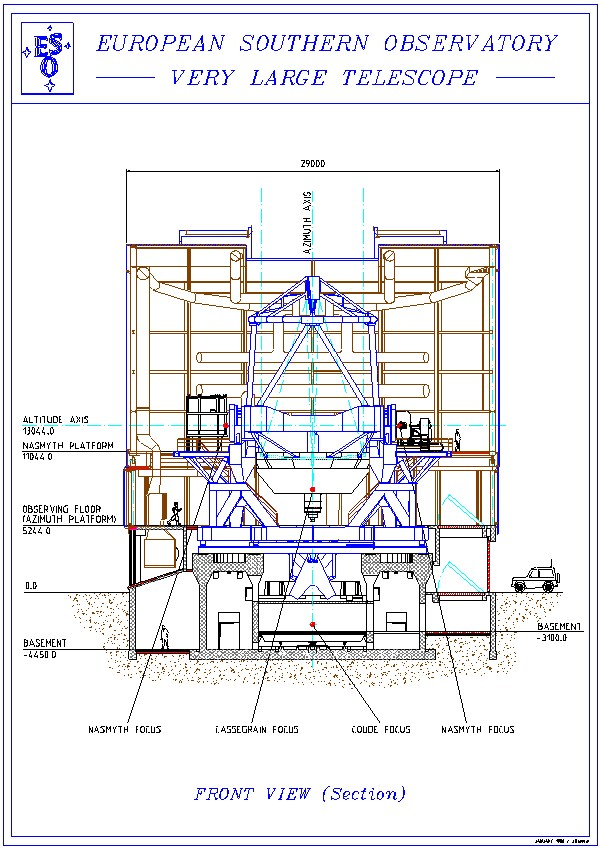
\includegraphics[width=6cm]{figures/front_ut.jpg}
\caption{\label{fig:front_ut} Diagrama frontal de un UT} Fuente: The VLT White Book \cite{eso1998vlt}
\end{figure}

\begin{figure}[h]
\centering
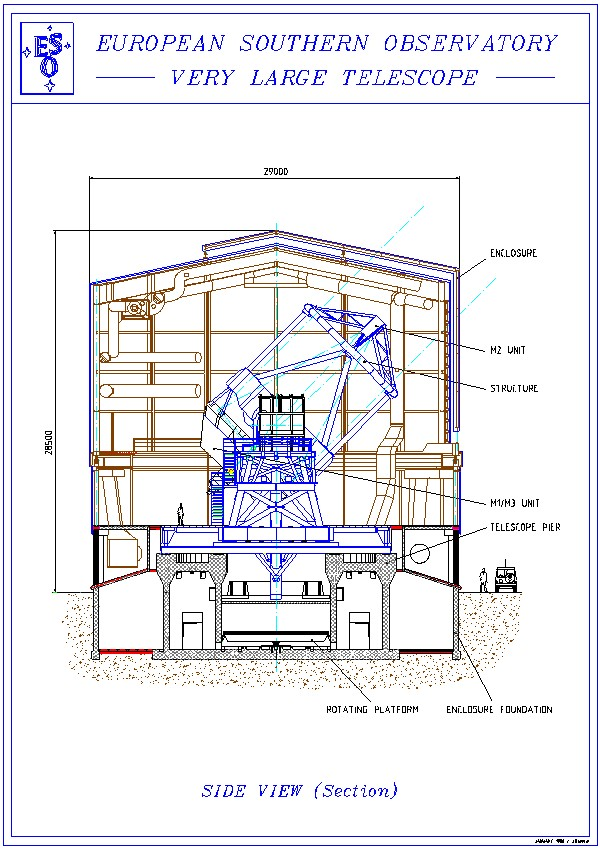
\includegraphics[width=6cm]{figures/side_ut.jpg}
\caption{\label{fig:side_ut} Diagrama lateral de un UT} Fuente: The VLT White Book \cite{eso1998vlt}
\end{figure}

\begin{figure}[h]
\centering
\includegraphics[width=8cm]{figures/real_ut.jpg}
\caption{\label{fig:real_ut} UT 2 visto desde el exterior} Fuente: Elaboración propia
\end{figure}

\begin{figure}[h]
\centering
\includegraphics[width=8cm]{figures/real_mount.jpg}
\caption{\label{fig:real_mount} Montura del M1} Fuente: Elaboración propia
\end{figure}

El M1 está compuesto de espejos más pequeñas, distribuidas en forma de dona. Bajo M1, repartidos en 6 anillos concéntricos, se encuentran 150 actuadores de fuerza axiales; estos son, pistones hidráulicos y neumáticos, donde cada actuador se encuentra debajo de una espejo pequeña respectiva. Estos actuadores dan a M1 una determinada forma óptica, determinada por el patrón de fuerza presentado por los actuadores \cite{eso1998vlt}. El M1 es visible en la Imágen \ref{fig:real_m1}.

\begin{figure}[h]
\centering
\includegraphics[width=8cm]{figures/real_m1.jpg}
\caption{\label{fig:real_m1} Espejo M1, con M2 reflejado y M3 en el centro} Fuente: Elaboración propia
\end{figure}

El M2 consiste de una espejo de 0.9 metros de diámetro, montada a una distancia de aproximadamente 12.3 metros de M1 a lo largo del eje azimutal, con la espejo de M2 apuntando hacia M1. El M2 además está montado sobre un mecanismo electromecánico que sujeta y controla su inclinación \cite{eso2011m2}. El M2 es visible en la Imágen \ref{fig:real_m2}.

\begin{figure}[h]
\centering
\includegraphics[width=8cm]{figures/real_m2.jpg}
\caption{\label{fig:real_m2} Espejo M2} Fuente: Elaboración propia
\end{figure}

El M3 consiste de una espejo elíptica de 1.24 metros de diámetro mayor con 0.86 metros de diámetro menor. Este se ubica dentro de una torre, posicionada en el orificio central del M1. Este puede rotar alrededor de su eje azimutal \cite{eso2011m1}. El M3 es visible en la Imágen \ref{fig:real_m3}.

\begin{figure}[h]
\centering
\includegraphics[width=8cm]{figures/real_m3.jpg}
\caption{\label{fig:real_m3} Espejo M3} Fuente: Elaboración propia
\end{figure}

\subsection{SISTEMA DE ÓPTICA ACTIVA}
La Óptica Activa es un sistema integrado en el M1, encargado de corregir las aberraciones y degradación en la calidad de imágen provocadas por las ópticas del espejo \cite{eso1998vlt}.

Estas aberraciones ópticas suelen ser causadas por la sensibilidad de este a perturbaciones ambientales, cómo las distorsiones térmicas, deformación de espejo por ráfagas de viento, errores de manufactura y mantenimiento del telescopio, entre otros. Esta sensibilidad es causada por la baja proporción entre el grosor y el diámetro del espejo, la cuál es la principal característica que permite al espejo M1 tener su gran tamaño, debido a que esta proporción es la que permite deformar el espejo \cite{wilson1987active}.

El ciclo básico del sistema de Óptica Activa se ilustra en la imágen del Anexo 1. El mismo sigue el siguiente procedimiento:

\begin{enumerate}
    \item El sensor de frente de onda Shack-Hartmann toma una imagen de una estrella en el cielo y la toma como guia\cite{eso1998vlt}.

    \item Se analiza la imágen y se miden las perturbaciones ópticas, calculando las aberraciones\cite{wilson1987active}.

    \item Cuando la desviación es considerable, se genera un set de fuerzas que se deben aplica al M1 para corregir las perturbaciones \cite{wilson1987active}.

    \item Se aplica el set de fuerzas al espejo M1 y, durante una observación, el sensor de frente de onda Shack-Hartmann toma una nueva imágen, repitiendo el proceso\cite{wilson1987active}. Un ejemplo de imágen tomada por el sensor Shack-Hartmann se muestra en la Imágen \ref{fig:sh}.

    \begin{figure}[h]
    \centering
    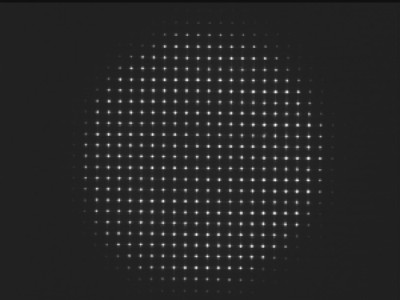
\includegraphics[width=8cm]{figures/sh_eje.png}
    \caption{\label{fig:sh} Imágen capturada por un sensor de frente de onda Shack-Hartmann} Fuente: Implementation of adaptive optics in fluorescent microscopy using wavefront sensing and correction\cite{azucena2010ao}
    \end{figure}

     \item Todo este ciclo es repetido hasta que la imágen tomada durante el Paso 1 venga con una calidad óptica\cite{wilson1987active}.

\end{enumerate}

\subsection{SENSOR DE FRENTE DE ONDA}
Un sensor de frente de onda es un dispositivo electrónico diseñado para calcular las aberraciones ópticas presentes en una imágen tomada, ya sea en el espectro visible o en infrarrojo. El VLT usa CCD Shack-Hartmann como sensores de frente de onda, con cada UT poseyendo uno en un brazo mecánico específico para los sensores.\cite{eso1998vlt}

El objetivo del uso de sensores Shack-Hartmann es la medición de distorsiones del frente de onda capturado desde la fuente, sobre las cuáles se realiza el proceso de Óptica Activa.\cite{eso1998vlt}

\subsection{LOGS}
Logging se refiere al proceso de registrar diferentes eventos y actividades que ocurren dentro de un sistema de software \cite{jayathilake2011mind}. Estos registros suelen almacenarse en archivos para su posterior análisis, tanto por parte de desarrolladores como de operadores externos.

Los registros de log son los únicos tipos de datos que, valga la redundancia, registran información de la operación interna de un sistema de software, por lo que su rol en la industria es importante. Debido a esto mismo, los registros de log pueden alcanzar tamaños en el orden de hasta el orden de millones de líneas\cite{ma2023automatic}.

Los registros de log de los telescopios UT registra un día completo de operación, donde se registra información sobre las condiciones ambientales, el funcionamiento del sistema de Óptica Activa, la toma de imágenes durante periodos de calibración y de observación, entre otros. Debido a lo anterior, estos registros de log suelen alcanzar el orden de cientos de miles de líneas. Un ejemplo de estos registros de log puede verse en el Anexo 2.

Las líneas de un registro de log estan compuestas de tokens estáticos y valores dinámicos. Los tokens estáticos corresponden a cadenas de texto que entregan metadata e información complementaria sobre el dato reportado en las líneas, y como tal se repiten de forma sistemática a lo largo del registro. Los valores dinámicos son cadenas de texto o números que entregan el valor del dato reportado, y por ende no se repiten con un patrón claro en el registro \cite{ma2023automatic}. 

\subsection{ANÁLISIS DE LOGS}
Originalmente, el análisis de registros de logs era realizado por desarrolladores con el fin de trazar el flujo de ejecución del sistema de software, identificar excepciones y potenciales errores. \cite{jayathilake2011mind}

Actualmente este enfoque se ha expandido a casos de uso en otros servicios en la industria \cite{ma2023automatic}, debido a que, por la naturaleza de la información contenida en los registros de log, su análisis permite a los operadores detectar, diagnosticar e incluso predecir errores que puedan afectar la disponibilidad y el rendimiento del sistema de software \cite{jayathilake2011mind}.

En el pasado, durante la prevalencia del enfoque original, el análisis de registros de log era realizado aplicando revisiones visuales y reglas construidas manualmente. Sin embargo, la complejidad de los sistemas de software actuales ha llevado a la complejización de sus respectivos registros de logs, por lo que ya no es posible depender solamente de los métodos anteriormente mencionados. \cite{ma2023automatic}

Por esto, en los últimos años se ha desarrollado ampliamente el área del análisis automatizado de registros de logs, mejorando su eficiencia y exactitud mediante la aplicación de tecnologías distribuidas y técnicas de machine learning. \cite{ma2023automatic}

\subsection{ESTRUCTURACIÓN DE LOGS}
Los registros de logs generalmente poseen una composición demasiado compleja como para ser interpretada de forma directa y manual; sin el acceso de conocimiento profesional, es difícil seleccionar de forma manual las reglas apropiadas para la comprensión de los registros de log \cite{ma2023automatic}. Por esta condición es que se refiere a que los registros de log sean “No Estructurados” o “Semi Estructurados”. 

Además, el gran tamaño de los archivos de log promedio también se vuelve un problema para el análisis manual de los registros de log \cite{ma2023automatic}.

Debido a esto, durante los últimos años, se han desarrollado herramientas, procedimientos y frameworks para el análisis automático de registros de log, y una parte considerable de los esfuerzos realizados se enfocan en la “Estructuración” de los registros de log.

Actualmente, el workflow de análisis automático de registros de log se divide en 2 etapas centrales \cite{ma2023automatic}:

\begin{itemize}
    \item Log Parsing: Se toman los registros semi-estructurados de log y se generan plantillas a partir de estos. Una plantilla es una sentencia estructurada que se repite entre varios registros de log, dividiéndose en los tokens estáticos y valores dinámicos. \cite{ma2023automatic}

    \item Feature Extraction: Se aplican las plantillas generadas sobre los registros de log para obtener las características, esto es, las variables dinámicas, de los mismos. \cite{ma2023automatic}

\end{itemize}

\subsection{ORIGENES DE DATOS}

Tres origenes de datos son considerados para la presente memoria:

\begin{enumerate}
    \item Registros de log: El origen de dato más importante para esta memoria, considerando la problemática a resolver. Estos datos son propios de los telescopios UT, y como tales, se obtienen directamente de los mismos una vez terminada su ejecución \cite{eso1998vlt}

    \item Imágenes en formáto fits: Las imágenes tomadas por el telescopio usan el formato fits, el cuál es universal en ciencias y astronomía\cite{nasa2025fits}. Es formato se divide en dos secciones: el contenido científico y el Header, donde este último contiene la metadata que describe a la misma imágen que lo aloja, como por ejemplo su número de ID, su tiempo de exposición, las fechas de inicio y término de grabado, entre otros\cite{nasa2025fits}. Para el caso de esta memoria, solo importan las imágenes que fueron tomadas desde el sensor de frente de onda como parte del ciclo de Óptica Activa.


    \item Observaciones en formáto csv: La ESO mantiene en una página web con el fin de archivar la información sobre todas las observaciones válidas de los UTs. Desde esa página se pueden obtener los datos de todas las observaciones de un día mediante una query. La información disponible en la página puede incluir el número de ID de la observación, la fecha de inicio, el tiempo de exposición, el instrumento de captura de la imágen, entre otros.

\end{enumerate}
\newpage
\secnumbersection{PROPUESTA DE SOLUCIÓN}

Se debe desarrollar la solución propuesta. Los subcapítulos por poner aquí son propios del autor. Se sugiere mencionar metodología usada. Es conveniente incorporar figuras y tablas para aclarar la solución, que deben indicar el número de la figura, su nombre y su autor o fuente (si las diseñas tú, la fuente es ``Elaboración propia''). Ver ejemplos en esta página y en la siguiente.

Cabe mencionar que aquí está la esencia del trabajo en lo que se refiere al aporte creativo del memorista, es el momento de demostrar que usted es un destacado profesional que creó, diseñó y/o llevó a cabo la solución propuesta.

\subsection{EJEMPLO DE COMO CITAR FIGURAS E ILUSTRACIONES}

Se colocó una imagen que se puede referenciar también desde el texto (Ver figura \ref{fig:malla}).

\begin{figure}[h]
\centering
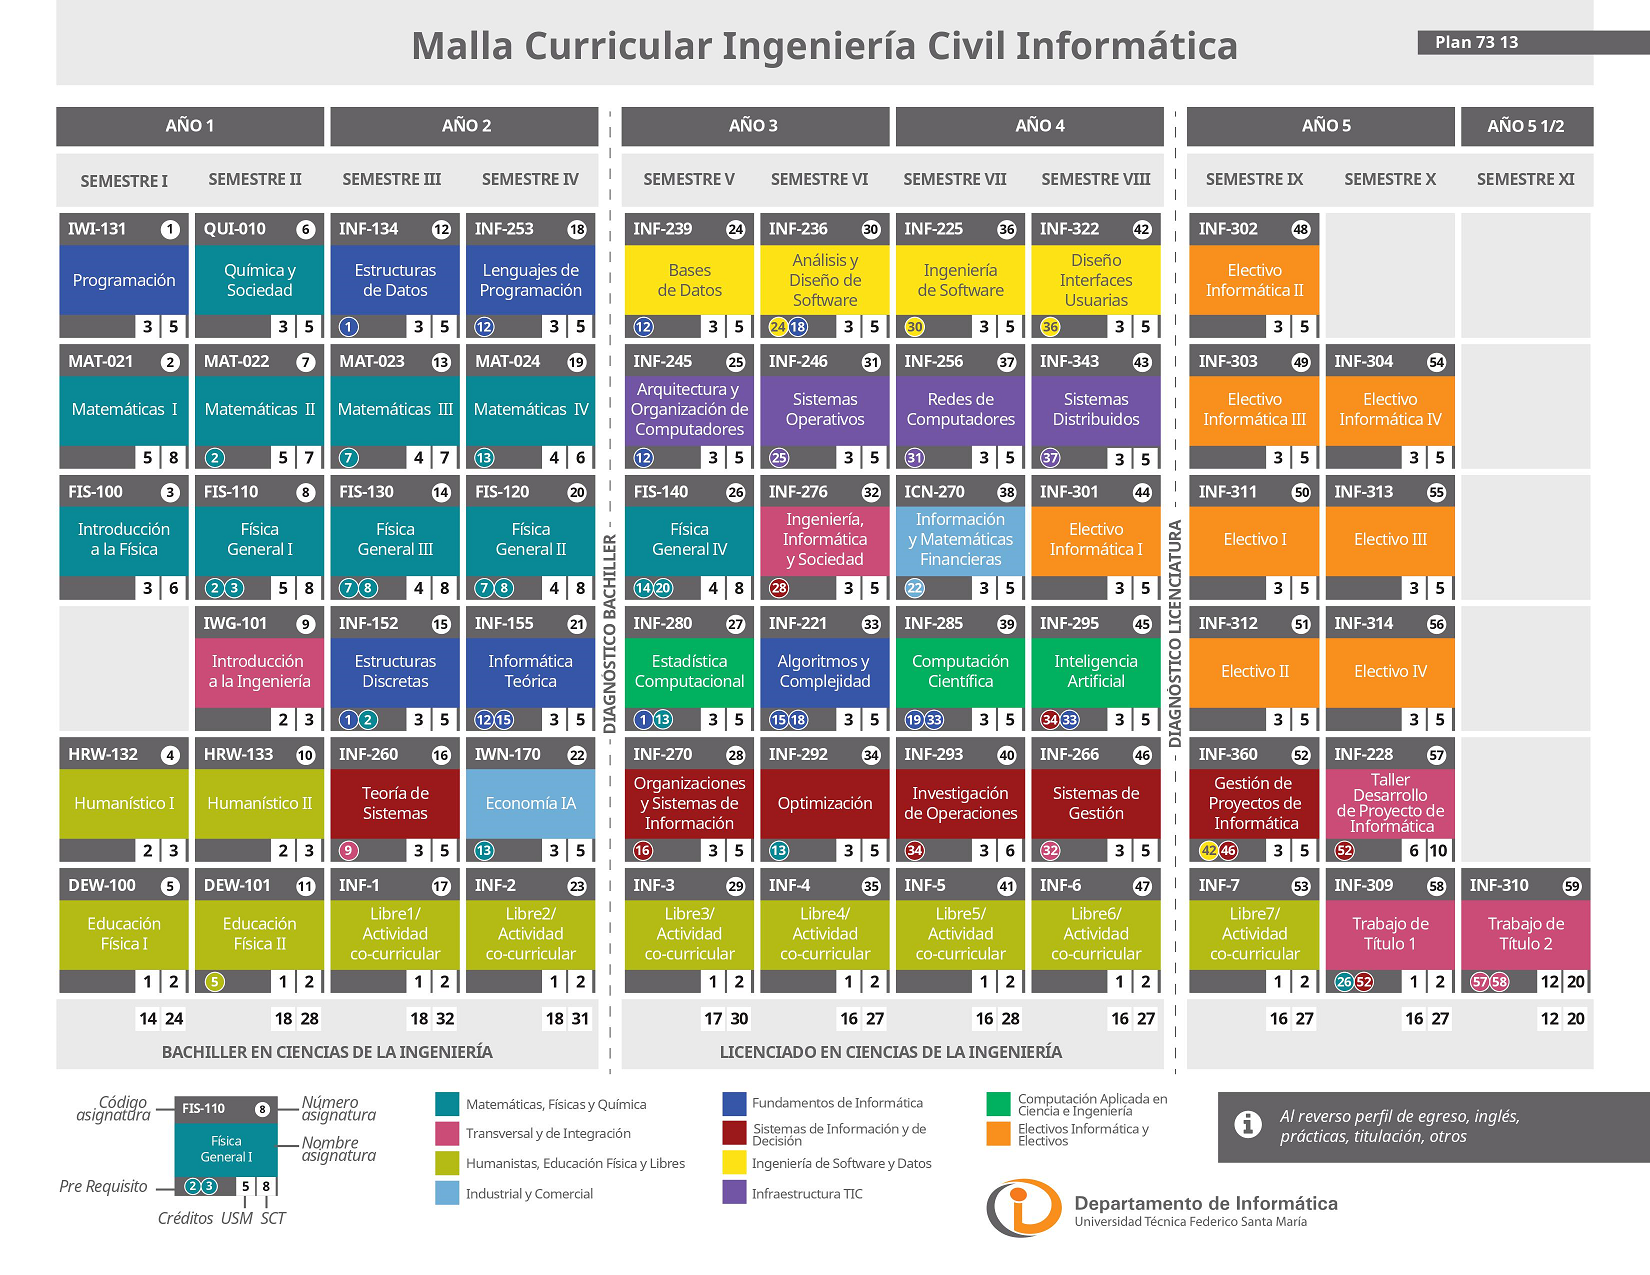
\includegraphics[width=0.8\textwidth]{malla_ingenieria_informatica}
\caption{\label{fig:malla} Malla Curricular Ingeniería Civil Informática.} Fuente: Departamento de Informática.
\end{figure}

\newpage
%\secnumbersection{VALIDACIÓN DE LA SOLUCIÓN}

\subsection{Algoritmo}

El algorimo final sigue el flujo detallado en el Anexo 3, el cuál fue detallado en el Capítulo 3. El mismo se divide en los siguientes pasos:

\subsubsection{Log Formatting}
Cumple con el proceso planteado en la sección 3.3.1, donde se remueven los tokens de fecha y hora iniciales, debido a su redundancia a nivel de línea, además de corregir otros detalles de formato con tal de facilitar el posterior análisis.

\subsubsection{Obs Filtering} 
Cumple con el proceso descrito en la sección 3.3.2, donde se obtiene un archivo csv con las observaciones de la noche seleccionada, para luego formar bloques de tiempo basados en los tiempos que tarda cada observaciones, más el efecto de parámetros de margen y unión, donde finalmente se filtran las líneas de log con tal de quedar solo con aquellas cuya fecha se encuentre dentro de alguno de esos bloques de tiempo.

\subsubsection{Log Parsing}
Cumple con el proceso descrito en la sección 3.4, donde a base de una archivo plano de plantillas, se itera sobre las líneas de log, aplicando cada plantilla por línea hasta encontrar alguna que calze y guardar la data extraída en un json final.

Como se mencionó en la sección 3.4.2, el método para realizar la extracción es mediante Expresiones Regulares, lo cuál se manifiesta tanto en el archivo de plantillas que se ingresa a la función, junto con las líneas a extraer, como en el método de extracción que se aplica a línea de log.

\subsubsection{Generate Dataframes} 
Cumple con el proceso de la sección 3.5.2, donde se menciona el traslado de los datos del json generado en la función anterior a un conjunto de dataframes, usando los campos \"group\" y \"label\" como etiquetas para reconocer a qué dataframe destinar los datos.

De esta función se generan 4 dataframes, como se señalo en la sección 3.5.1: df\_corrections, para las instancias de corrección; df\_images, para las imágenes capturadas; df\_f\_dist, para las distribuciones de fuerza de los actuadores; y df\_additional\_data, para los datos adicionales relacionados con la Óptica Activa.

\subsubsection{Validate Forces} 
Cumple con el segundo item de la sección 3.5.3, donde se especifica la validación de los datos dentro de df\_f\_dist generado en la función anterior. 

Principalmente, se eliminan los datos con ID\_f\_dist nulo, además de remover aquellos que no sean antecedidas y/o seguidas por imágenes únicas.

\subsubsection{Validate Images} 
Cumple con el tercer item de la sección 3.5.3, donde se especifica la validación de los datos dentro de df\_images generados en la función anterior. Solamente se eliminan aquellos datos con ID\_image nulo.

\subsubsection{Link Images} 
Cumple con el requisito de la sección 3.5.1, sobre df\_images manteniendo la dirección local del archivo .fits correspondiente como un atributo de los datos del dataframe.

En esta función, se ingresa a la carpeta donde estan almacenados los archivos .fits, se extrae el número de ID y el tiempo de exposición del header de cada .fits y se usan estos para buscar el dato de df\_images que le sea correspondiente. En caso de encontrarlo, se guarda su dirección local en el atributo correspondiente del dato.

\subsubsection{Validate Corrections} 
Cumple con el primer item de la sección 3.5.3, donde se especifica la validación de los datos dentro de df\_corrections generado en la función anterior.

Principalmente se eliminan los datos con ID\_corr nulo, además de remover aquellos sin distribución de fuerza posterior a la corrección.

\subsubsection{Link Dataframes}
Cumple con el proceso descrito en la sección 3.5.4, en la que se indica como calzar los datos de un dataframe con los datos de dataframe df\_corrections mediante los timestamp de estos datos, comparando estos para luego copiar la ID del dato de la cantidad deseada en un campo designado dentro del dato correspondient en df\_corrections.

Para esta función, como la construcción de relaciones entre df\_images con df\_corrections y entre df\_f\_dist con df\_corrections es identico, por lo que se pudo generalizar y paramétrizar esta construcción en una misma función, que varía con el dataframe de la cualidad deseada, el nombre de la cualidad deseada y el campo de tiempo dentro del dataframe, como parámetros de entrada.

\subsection{Ejecución}

Para ejecutar el código desarrollado, se debe entregar la fecha y el número del UT, en ese orden, del registro a analizar. Para el apropiado funcionamiento del algoritmo, el archivo de log debe estar previamente cargado en el sistema local.

Además se desarrolló un sistema de flags opcionales que otorga la posibilidad de habilitar o deshabilitar las funciones descritas en la sección 4.2.1. Estas se pueden ver en \ref{myverbatim:flags}.

\begin{myverbatim}[caption={Flags del codigo},label={myverbatim:flags}]
usage: poc-final-v2.py [-h] [-t TEMPLATEFILE] 
[-p] [-o] [-i] [-l] [-c] [-s SAVE] [-r] date ut

positional arguments:
  date              Date to analyzed
  ut                Number of the UT telescope to be analyzed

options:
  -h, --help        show this help message and exit
  -t TEMPLATEFILE, --templatefile TEMPLATEFILE
                    Path to the text file where the templates
                    are stored (if no name is written, 
                    ./poc_templates.txt
                    will be set by default)
  -p, --preprocess  Skips logs pre-processing stage: removal
                    of log headers and grouping of log 
                    lines in sections, based on when 
                    AG GUIDE has stopped activity
  -o, --obsprocess  Skips observation files processing stage: 
                    filtering of log lines based on time 
                    intervals where a valid observation has 
                    been performed
  -i, --linkimages  Skips linking of image log data with 
                    fits files: write of the fits files' 
                    path respective to each image row 
                    in the images' dataframe
  -l, --linkdataframes  Skips linking of correction 
                        dataframe with related dataframes: 
                        write of the ids of the force 
                        distribution and image respective 
                        to each row in the correction 
                        dataframe
  -c, --console     Prints resulting dataframes on console
  -s SAVE, --save SAVE Stores resulting dataframes in 
                        csv files
  -r, --report      Prints a report detailing the processing 
                    of log lines
\end{myverbatim}

Existen 2 posibles modos de retorno de los dataframes generados: por consola o por csv. Estos se habilitan con las flags -c y -s, respectivamente.

\subsection{Pruebas}

Para corroborar el correcto funcionamiento del algoritmo, es necesario analizar los resultados del mismo, junto con revisar el rendimiento y exactitud de la ejecución.

\subsubsection{Metodología}

Para poder analizar el desempeño y resultados del algoritmo, primero se realiza un conteo manual de las instancias de corrección, las distribuciones de fuerza y las imagenes presenten en una muestra de archivos de log. Luego, se ejecuta el algoritmo para procesar los mismos archivos de log, y se comparan los resultados. 

La muestra se compone de los siguientes archivos de log:

\begin{itemize}
    \item L1 : Archivo de log para la observación del UT 1 durante la noche del 04/08/2025.

    \item L2 : Archivo de log para la observación del UT 1 durante la noche del 05/08/2025.

    \item L3 : Archivo de log para la observación del UT 3 durante la noche del 04/08/2025.

    \item L4 : Archivo de log para la observación del UT 3 durante la noche del 05/08/2025.

    \item L5 : Archivo de log para la observación del UT 4 durante la noche del 04/08/2025.

    \item L6 : Archivo de log para la observación del UT 4 durante la noche del 05/08/2025.    
\end{itemize}

Una vez realizadas las ejecuciones, se procede a analizar las estadísticas de los resultados, más específicamente el número de instancias de corrección, distribución de fuerzas e imágenes obtenidas, además del tiempo de ejecución.

Este proceso de revisión se realizará primero en ámbitos generales del algoritmo, y luego se revisará para cada etapa de forma más específica.

\subsubsection{Resultados generales}

Los resultados encontrados de forma manual para cada archivo de log se refleja en la Tabla \ref{table:manual}. Luego, las cantidades encontradas en los mismos archivos por el algoritmo se encuentran en la Tabla \ref{table:auto}.


\begin{table}[h]
    \centering
    \caption{\label{table:manual} Cantidades encontradas de forma manual}
    \begin{tabular}{|p{2.8cm}|p{2.8cm}|p{2.8cm}|p{2.8cm}|p{2.8cm}|}
        \hline
        Log & Líneas & Correcciones & Fuerzas & Imagenes \\
        \hline
        L1 & 427195 & 626 & 586 & 851 \\
        \hline
        L2 & 384729 & 598 & 562 & 802 \\
        \hline
        L3 & 409830 & 537 & 277 & 908 \\
        \hline
        L4 & 371450 & 546 & 262 & 741 \\
        \hline
        L5 & 444126 & 491 & 287 & 786 \\
        \hline
        L6 & 422312 & 495 & 358 & 713 \\
        \hline
    \end{tabular}
\end{table}


\begin{table}[h]
    \centering
    \caption{\label{table:auto} Cantidades encontradas por el algoritmo}
    \begin{tabular}{|p{2.3cm}|p{2.3cm}|p{2.3cm}|p{2.3cm}|p{2.3cm}|p{2.3cm}|}
        \hline
        Log & Líneas & Correcciones & Fuerzas & Imagenes & Tiempo (en segundos) \\
        \hline
        L1 & 427195 & 4 & 5 & 11 & 61.92 \\
        \hline
        L2 & 384729 & 31 & 33 & 54 & 89.33 \\
        \hline
        L3 & 409830 & 4 & 5 & 8 & 69.49 \\
        \hline
        L4 & 371450 & 19 & 19 & 46 & 79.14 \\
        \hline
        L5 & 444126 & 3 & 3 & 4 & 59.18 \\
        \hline
        L6 & 422312 & 18 & 18 & 31 & 103.25 \\
        \hline
    \end{tabular}
\end{table}

Es evidente la amplia diferencia entre ambas cantidades, sin embargo, existen motivos para explicarlo.

Primero, se debe mencionar que la extracción manual se realizó mediante un simple conteo de lineas de log según ciertos tokens clave, mientras que para la extracción con el algoritmo se aplicó lógica durante las validaciones y filtros que permiten un conteo con información más certera, aunque reducida en tamaño.

Ejemplos de reglas incumplidas en los logs: se ha visto que en los registros de log, existen varias fotos que se pueden tomar consecutivamente en lapsos de unos pocos segundos; distribuciones de fuerza que no son anticipados ni seguidos directamente por una toma de imágen; entre otros. Estos casos, son detectados por el algoritmo, evitando la extracción de estos datos extra.

El otro motivo de porque la diferencia en el número de cantidades es la filtración por observación: la cantidad de observaciones totales es baja, lo cuál inmediatamente deja fuera a una buena parte de las cantidades presentes en el archivo de log.

Ahora bien, como se menciono en la sección 3.3.2, el filtro de observaciones se realiza con tres parámetros: el margen inferior y el margen superior para cada bloque de tiempo, y el umbral de unión entre bloques de tiempo. Estos tienen sus valores asignados de forma rígida dentro del código. Por ende, la modificación de estos parámetros ampliaría el rango de búsqueda de las cantidades en el archivo de log. Actualmente, se definieron los margenes anterior y posterior como 10 segundos cada uno, y el umbral de unidad de los bloques de observación se encuentra en 30 segundos.

Es posible aumentar estos paramétros, sin embargo tampoco se pueden llegar a extremos muy altos, ya que puede comenzar a presentar ruido por el sobrelape de bloque de tiempo de las observaciones.

\subsection{Resultados para Filtrado de líneas de log}

Parte crucial de este etapa es el cruce de los registros de log con los datos de observaciones, con tal de filtrar los primeros, tal como se explicó en la sección 3.4.2. Con esto en mente, se puede examinar el rendimiento de esta etapa comparando la cantidad de líneas de log que ingresa con la cantidad que sale, para cada uno de los casos descritos al inicio de esta sección.

Los resultados de estas pruebas se exponen en la Tabla \ref{table:etapa1}


\begin{table}[h]
    \centering
    \caption{\label{table:etapa1} Cantidad de líneas de log filtradas}
    \begin{tabular}{|p{3.5cm}|p{3.5cm}|p{3.5cm}|p{3.5cm}|}
        \hline
        Log & Líneas entrada & Líneas salida & Porcentaje reducción \\
        \hline
        L1 & 427195 & 3829 & 99.10\% \\
        \hline
        L2 & 384729 & 23475 & 93.90\% \\
        \hline
        L3 & 409830 & 4496 & 98.90\% \\
        \hline
        L4 & 371450 & 22048 & 94.06\% \\
        \hline
        L5 & 444126 & 3593 & 99.19\% \\
        \hline
        L6 & 422312 & 27365 & 93.52\% \\
        \hline
    \end{tabular}
\end{table}

Se puede notar de inmediato el peso de los filtros en esta etapa: en todos los casos probados se redujo el número de líneas de log en más de un 90\%.

Esto trae ventajas y desventajas: por un lado, se asegura que las líneas de log que pasen a la etapa de Extracción de Datos correspondan a observaciones válidas del telescopio; por el otro lado, es posible teorizar que se están desechando líneas de log que puedan poseer información relacionada con la ejecución del sistema de Óptica Activa.

\subsection{Resultados para Extracción de los datos}

Se prueban los dos métodos de extracción mencionados en la sección 3.4.2, usando la serie de parámetros iniciales señalados en el inicio, y se registran los tiempos y cantidad de datos extraídos para cada método:

\begin{table}[h]
    \centering
    \caption{\label{table:etapa2} Tiempos y cantidad de datos para modos de extracción}
    \begin{tabular}{|p{2cm}|p{3cm}|p{3cm}|p{3cm}|p{3cm}|}
        \hline
        Log & Datos TTP & Tiempo TTP (en segundos) & Datos Regex & Tiempo Regex (en segundos) \\
        \hline
        L1 & 64 & 156.56 & 68 & 61.92 \\
        \hline
        L2 & 533 & 636.70 & 546 & 89.33 \\
        \hline
        L3 & 59 & 138.05 & 62 & 69.49 \\
        \hline
        L4 & 441 & 569.63 & 450 & 79.14 \\
        \hline
        L5 & 31 & 144.02 & 34 & 59.18 \\
        \hline
        L6 & 462 & 710.65 & 473 & 103.25 \\
        \hline
    \end{tabular}
\end{table}

Con esta prueba, se puede notar que ambos métodos de extracción retornan cantidades similares de datos, sin embargo TTP toma una mayor cantidad de tiempo en comparación con Regex. Más particularmente, se puede notar que para los casos con decenas de datos, el método con TTP tardaba más del doble que el método con Regex, mientras que en los casos con cientos de datos, el método de TTP tarda alrededor de 7 veces más que el método de Regex.

Con esta prueba, se decide escoger el método de extracción con Regex por sobre el método de extracción usando TTP, basándose exclusivamente en la velocidad del método de extracción predilecto.

Una vez determinado el método de extracción, se procede a determinar la cantidad de líneas cuyos datos fueron extraídos sobre la cantidad de líneas que ingresaron a la etapa, similar a la prueba realizada para Filtrado de Líneas de Log. Los resultados se muestran en la Tabla \ref{table:etapa2c2}

Esto se revisa en esta etapa porque, si bien aquí no tiene el fin de filtrar directamente, esto igualmente ocurre frecuentemente debido a la aplicación de plantillas, donde aquellas líneas de log que no calzen con ninguna plantilla serán descartadas.


\begin{table}[h]
    \centering
    \caption{\label{table:etapa2c2} Cantidad de líneas de log extraídas}
    \begin{tabular}{|p{3.5cm}|p{3.5cm}|p{3.5cm}|p{3.5cm}|}
        \hline
        Log & Líneas entrada & Líneas salida & Porcentaje reducción \\
        \hline
        L1 & 3829 & 135 & 96.47\% \\
        \hline
        L2 & 23475 & 940 & 95.99\% \\
        \hline
        L3 & 4496 & 142 & 96.84\% \\
        \hline
        L4 & 22048 & 819 & 96.29\% \\
        \hline
        L5 & 3593 & 73 & 97.97\% \\
        \hline
        L6 & 27365 & 806 & 97.05\% \\
        \hline
    \end{tabular}
\end{table}


Según lo reflejado en la Tabla \ref{table:etapa2c2}, los porcentajes de reducción son incluso mayores que en la etapa anterior, donde no bajan del 95\%.

Sin embargo, a diferencia de la etapa anterior, estos porcentajes altos no comprometen la cantidad de datos extraídos; por el contrario, son un sintoma esperable del proceso de aplicación de plantillas.

Para ilustrar esta defensa, se analizan los logs de operación del algoritmo, donde se destacan campos desechados durante la etapa de extracción. Los resultados para cada caso se presenta en la Tabla \ref{table:etapa2c3}.


\begin{table}[h]
    \centering
    \caption{\label{table:etapa2c3} Perdidas de datos durante extracción}
    \begin{tabular}{|p{3.5cm}|p{3.5cm}|p{3.5cm}|p{3.5cm}|}
        \hline
        Log & Corrección perdidas & Fuerzas perdidas & Imágenes perdidas \\
        \hline
        L1 & 2 & 0 & 0 \\
        \hline
        L2 & 2 & 0 & 0 \\
        \hline
        L3 & 3 & 0 & 0 \\
        \hline
        L4 & 20 & 0 & 0 \\
        \hline
        L5 & 0 & 0 & 0 \\
        \hline
        L6 & 17 & 0 & 0 \\
        \hline
    \end{tabular}
\end{table}

Incluso para el caso de L4 y L6, donde se pierden más datos en la tabla, son cantidades menores en comparación a los datos que extraen exitosamente (referidos en la Tabla \ref{table:etapa2}).

\subsection{Resultados para Guardado de los datos}

Similar a las etapas anteriores, se va a comparar la cantidad de datos que entran a la etapa con la cantidad de datos que salen de la misma. 

Solo se contarán datos de dsitribución de fuerzas, instancias de corrección e imágenes tomadas. Esto porque en esta etapa se realizan validaciones que pueden eliminar datos dependiendo del contexto, y dichas validaciones solo se aplican a esos tipos de datos.

Los resultados de este análisis se presentan en la Tabla \ref{table:etapa3}


\begin{table}[h]
    \centering
    \caption{\label{table:etapa3} Cantidad de datos filtrados}
    \begin{tabular}{|p{3.5cm}|p{3.5cm}|p{3.5cm}|p{3.5cm}|}
        \hline
        Log & Datos entrada & Datos salida & Porcentaje reducción \\
        \hline
        L1 & 26 & 20 & 30\% \\
        \hline
        L2 & 146 & 118 & 19.18\% \\
        \hline
        L3 & 24 & 18 & 25\% \\
        \hline        
        L4 & 116 & 84 & 27.59\% \\
        \hline
        L5 & 14 & 10 & 40\% \\
        \hline
        L6 & 100 & 67 & 33\% \\
    \end{tabular}
\end{table}

Si bien presenta bajas enlos números de datos, son porcentajes menores a los presentes en las etapas anteriores. Es posible que estas bajas sean causados por las validaciones, como se menciono anteriormente, considerando que en dichas validaciones se remueven valores con nulidad o que no cumplan con el orden distribución de fuerza - imágen establecido.
%\newpage
%\secnumbersection{CONCLUSIONES}

Las Conclusiones son, según algunos especialistas, el aspecto principal de una memoria, ya que reflejan el aprendizaje final del autor del documento. En ellas se tiende a considerar los alcances y limitaciones de la propuesta de solución, establecer de forma simple y directa los resultados, discutir respecto a la validez de los objetivos formulados, identificar las principales contribuciones y aplicaciones del trabajo realizado, así como su impacto o aporte a la organización o a los actores involucrados. Otro aspecto que tiende a incluirse son recomendaciones para quienes se sientan motivados por el tema y deseen profundizarlo, o lineamientos de una futura ampliación del trabajo.

\underline{Todo esto debe sintetizarse en al menos 5 páginas.}


\newpage
\secnumberlesssection{ANEXOS}

\begin{itemize}
    \item Anexo 1:
        \\
        \vspace{3.5cm}
        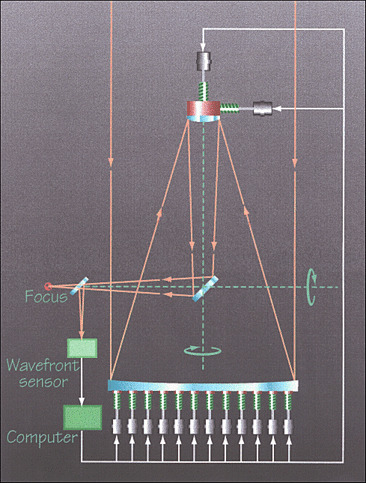
\includegraphics[width=6cm,height=9cm]{figures/actopt2.jpg} \\
        \vspace{3.5cm}


    \item Anexo 2:
        \\
        \vspace{3.5cm}
        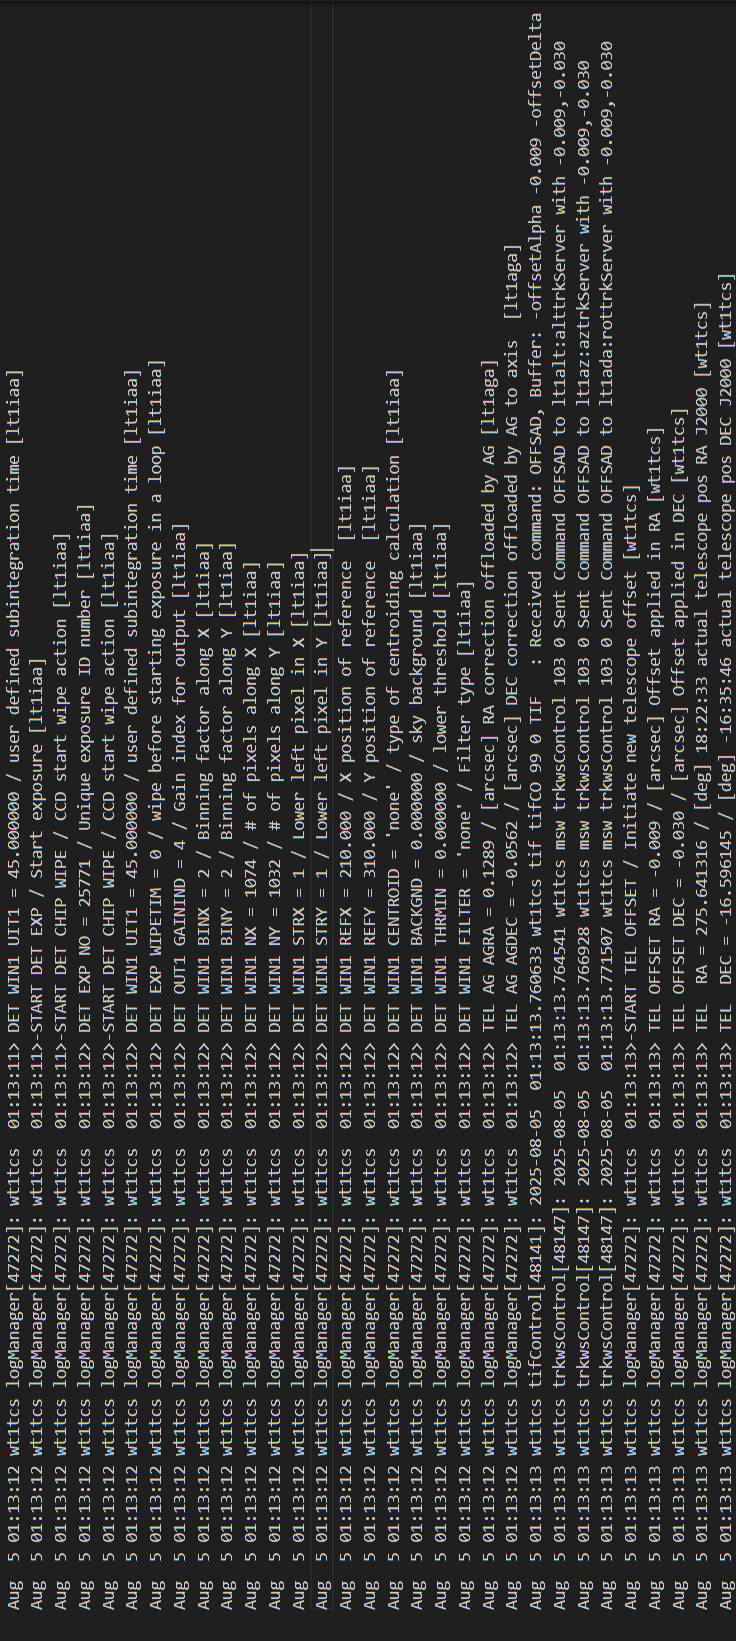
\includegraphics[width=12cm,height=18cm]{figures/log_vertical.png} \\
        \vspace{3.5cm}

    \item Anexo 3:
        \\
        \\
        \vspace{3.5cm}
        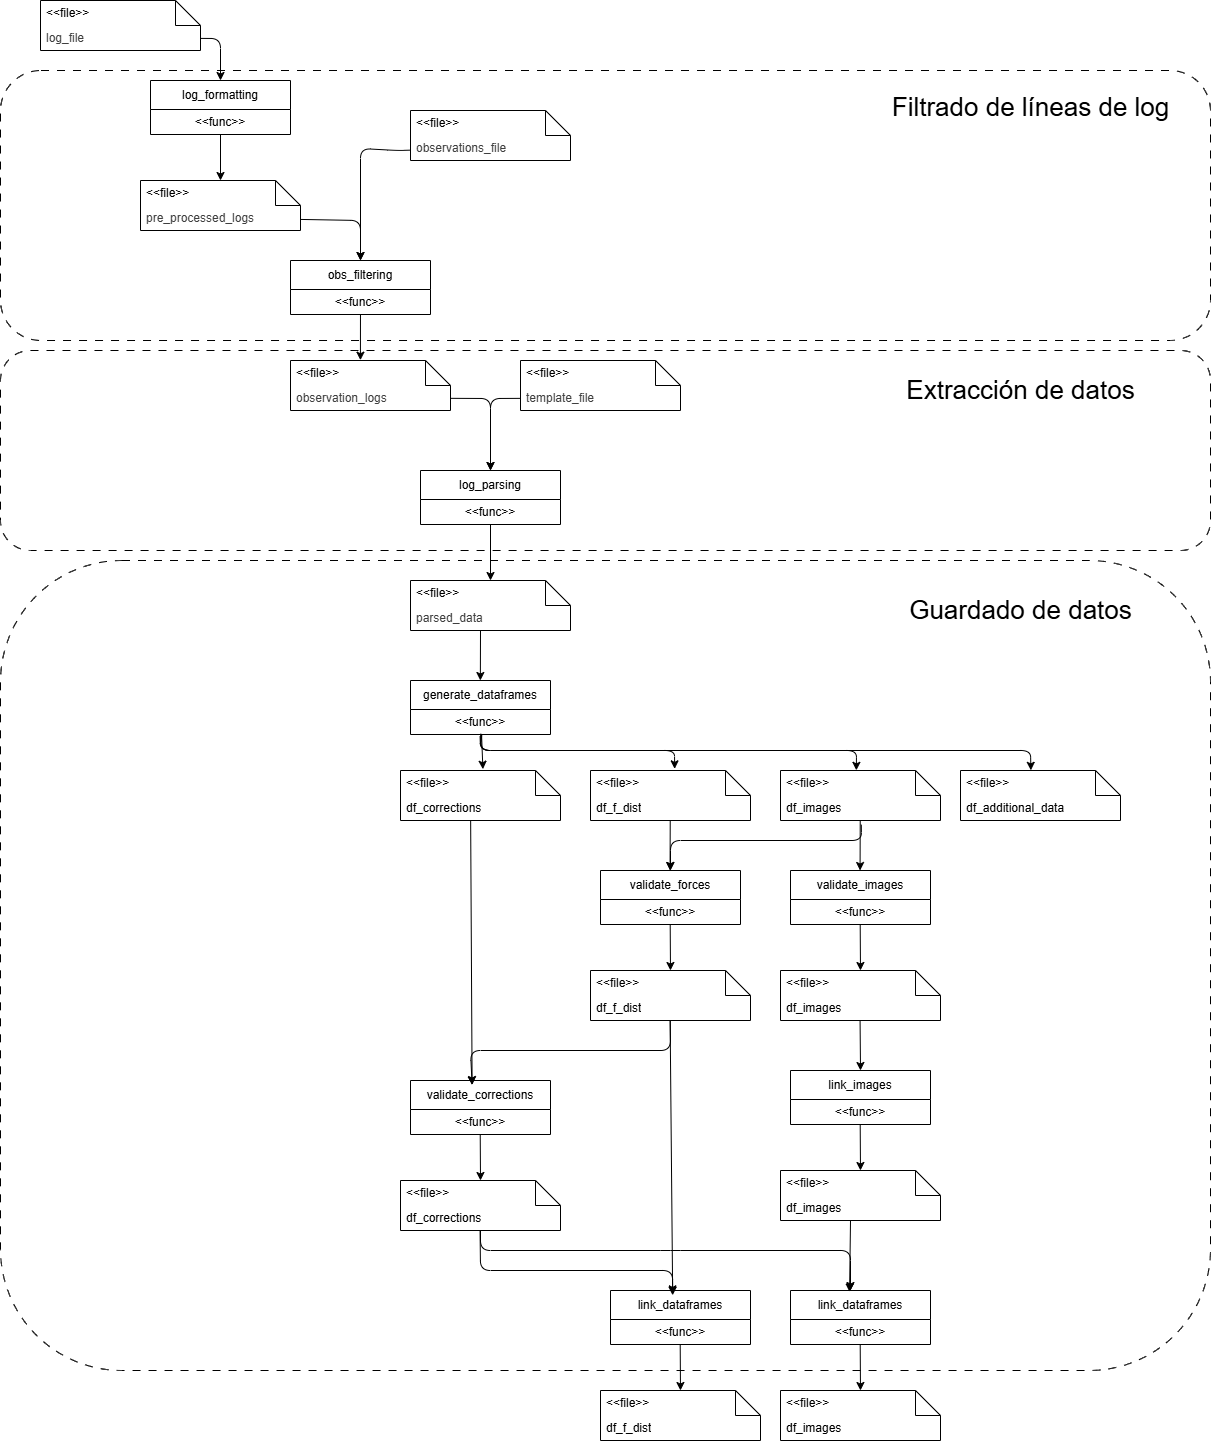
\includegraphics[width=12cm,height=16cm]{figures/flow_diagram.png} \\
        \vspace{3.5cm}

    \item Anexo 4:
        \\
        \\
        \vspace{3.5cm}
        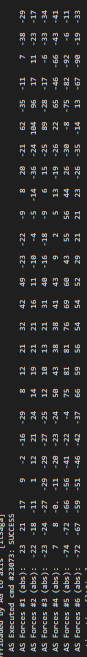
\includegraphics[width=2cm,height=16cm]{figures/log_f_dist.png} \\
        \vspace{3.5cm}
\end{itemize}


\begin{itemize}
    \item Diccionario 1: Frente de Onda

    El frente de onda es una superficie imaginaria que representa los puntos correspondientes de una onda que vibra al unisono. Cuando ondas idénticas con un origen en común viajan a través de un medio homogéneo, los senos y picos correspondientes a cada uno se mantienen en fase \cite{britannica2022front}. 

    \item Diccionario 2: Sensor de frente de onda

    Es un sensor diseñado para calcular las aberraciones de una imágen mientras se toma la misma. Generalmente las aberraciones son producidas por ladeos en los frentes de onda, presentes en imágenes que capturan objetos al otro lado de la atmósfera \cite{platt2001sh}

     \item Diccionario 3: Librería Template Text Parser

     Template Text Parser, o TTP, es una librería de Python que permite la extracción de datos de texto semi estructurado usando plantillas, manteniendo un rendimiento relativamente rápido. Iniclamente fue desarrollado para permitir el acceso procedural a datos producidos por las consolas de aparatos de red, sin embargo, actualmente puede ser usada para extraer cualquier texto semi estructurado que contenga patrones de repetición distintivos \cite{dmulyalin2021ttp}.
\end{itemize}

\newpage
% Bibliografía estilo APA:
\bibliographystyle{apalike-es}
\bibliography{bibliografia}{}

\end{document}
